\chapter{AF}
\label{chap:salvo}
\section{Problem}

% motivation
% explain fluro method
% explain skin model
% explain nelder mead
% explain filter choice

% results in "2d" 
% results in 3d + higher
% future work


\section{Nelder-Mead method}

The \gls*{nm} method is an algorithm for unconstrained optimisation. 
The algorithm is based upon iteratively updating a simplex. 
A simplex is a structure in $n-dimensional$ space, consisting of $n+1$ points that are not in the same plane. 
Therefore in 1D, the simplex is a line, in 2D a triangle, in 3D a tetrahedron, etc.. 
The Nelder-Mead method is a gradient free method, meaning that it does not require derivative to be calculated and that the search space does not need to be smooth.

The algorithm works by removing the worst vertex of the simplex and replacing it with a `better' vertex calculated via a number of different operations.
These operations can be seen in~\cref{fig:NM-operations}.

The first step of the~\gls*{nm} method is to sort the initial vertices according to their fitness.
For $n=2$, we define $x_w$ as the `worst' point, $x_l$ and the `lousy' point, and $x_b$ the `best' point, such that $f(x_b)\leq f(x_l)\leq f(x_w)$, where $f(x)$ is evaluating the `fitness' of a point $x$.
With the vertices sorted, the centroid of the simplex is calculated as in~\cref{eqn:centroid}.
The centroid is the mean of all the vertices bar the `worst' point.

\begin{figure}[!htbp]
    \centering
    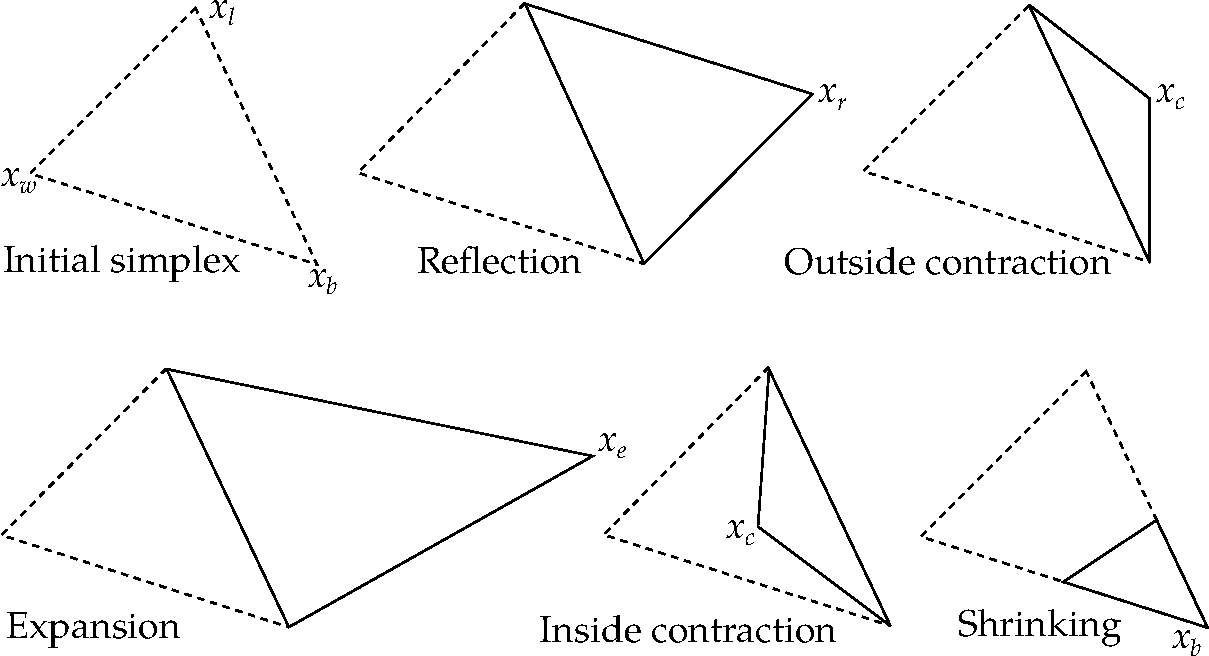
\includegraphics[width=0.75\textwidth]{simplex-operations.pdf}
    \caption{Operations that can be preformed on a simplex for $n=2$.}
    \label{fig:NM-operations}
\end{figure}

The next step is to move the simplex via a reflection.
To calculate the new vertex via reflection~\cref{eqn:reflect} is used, where $\alpha$ is the reflection factor.
If this new point, $x_r$, is better\footnote{Here better means the point has a lower fitness score, as we use $\chi^2$ metric to assess the fitness of a point.} than the current `best' point then we calculate a new point in the same direction but further using the expansion operation~\cref{eqn:expand}, where $\gamma$ is the expansion factor.
If this new point, $x_e$, is better than the `best' point then we replace $x_w$ with $x_e$ and start the process again.
However is $x_e$ is not better than the `best' point, then we discard it and replace the worst point with $x_r$ the reflected point.

If when calculating $x_r$, we find that is worse than the `best' point, we then check if $x_r$ is better than the `lousy' point.
If $x_r$ is better than $x_l$ then we replace the `worst' point and start the process again.
However if the $x_r$ is worse than $x_l$, we then compare it to the `worst' point.
If $x_r$ is better than the `worst' point then we preform and inside contraction~\cref{eqn:insidecontract}, where $\beta$ is the contraction factor.
If this new point, $x_{ic}$, is better than the `worst' point then we keep it, otherwise we preform the shrink operation, shrinking the whole simplex around the `best' point.

If $x_r$ is not worse than the `worst' point then we preform an outside contraction~\cref{eqn:outsidecontract}.
This computes a new point $x_{oc}$.
If $x_{oc}$ is better than $x_w$, then we keep it, otherwise again we shrink around the `best' point.

The process described above is summarised in~\cref{fig:NM-algo}.
Standard values for the factors are: $\alpha=1$, $\beta=\frac{1}{2}$, and $\gamma=2$.
Though in practise these values are adjusted for the problem at hand.

\begin{align}
c &= \frac{1}{n}\sum \limits_{i=1,i\neq w}^{n+1} x_i \label{eqn:centroid}\\
x_r &= c + \alpha(c - x_w)\label{eqn:reflect}\\
x_e &= c + \gamma(x_r - c)\label{eqn:expand}\\
x_{oc} &= c + \beta(x_r - c)\label{eqn:outsidecontract}\\
x_{ic} &= c + \beta(x_w - c)\label{eqn:insidecontract}
\end{align}

\begin{figure}[!htbp]
    \centering
    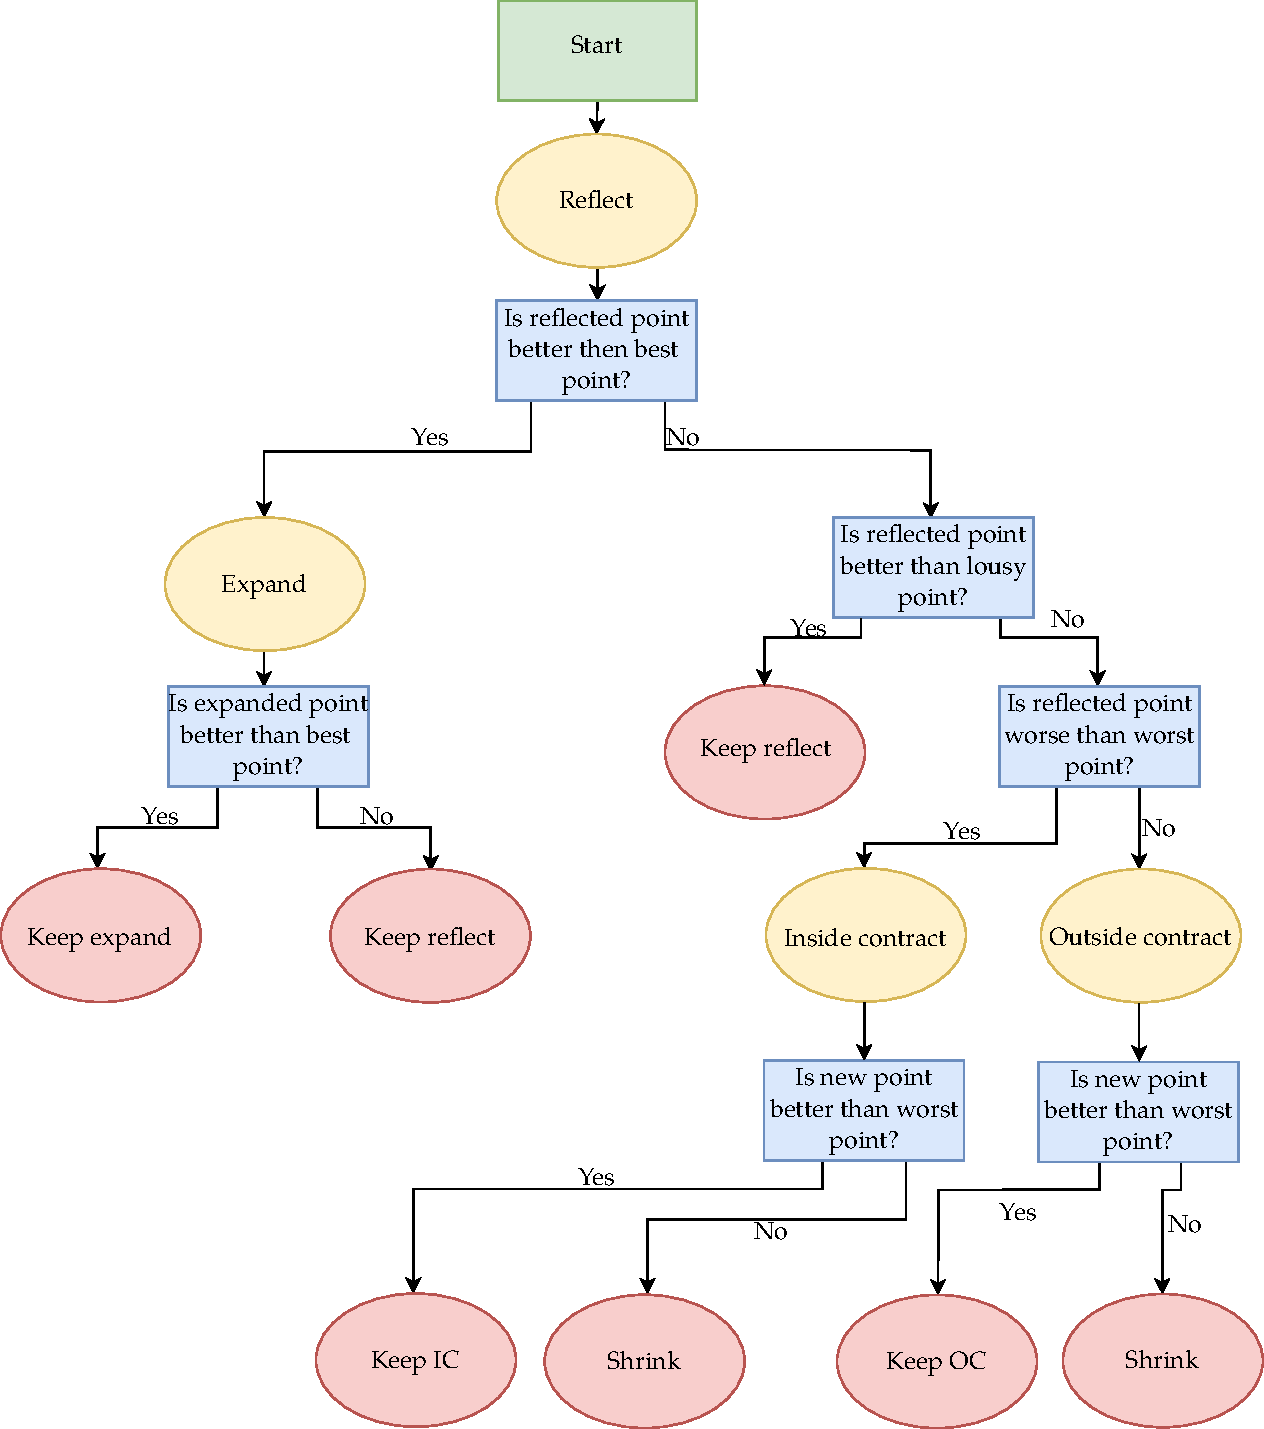
\includegraphics[width=0.65\textwidth]{flowchart.pdf}
    \caption{Nelder-Mead decision tree}
    \label{fig:NM-algo}
\end{figure}


The~\gls*{nm} method was coded in Fortran, so that it could be easily interfaced with the~\gls*{mcrt} code developed as part of this thesis.
To test that the method works as intended a number of trial functions were tested.


\begin{table}[]
    \begin{tabular}{c|c|c|c}
        Name                  & Formula                          & Global Minumum & Domain                    \\ \hline
        Sphere       & $x^2+y^2$                 & $f(0,0)=0.$     & $-\infty \leq x,y \leq \infty $ \\
        Rosenbrock   & $(a-x)^2+b(y-x^2)^2$      & $f(1,1)=0.$     & $-5 \leq x,y \leq 10 $ \\
        Himmelblau's & $(x^2+y-11)^2+(x+y^2-7)^2$ & $f(3,2)=0., $  & $-6 \leq x,y \leq 6$     \\
        & & $f(-2.805118,3.131312)=0.,$ &\\
        & & $f(-3.779310,-3.283186)=0.,$&\\  
        & & $f(3.584428,-1.848126)=0.$&
    \end{tabular}
\end{table}

\begin{figure}[!htbp]
    \centering
    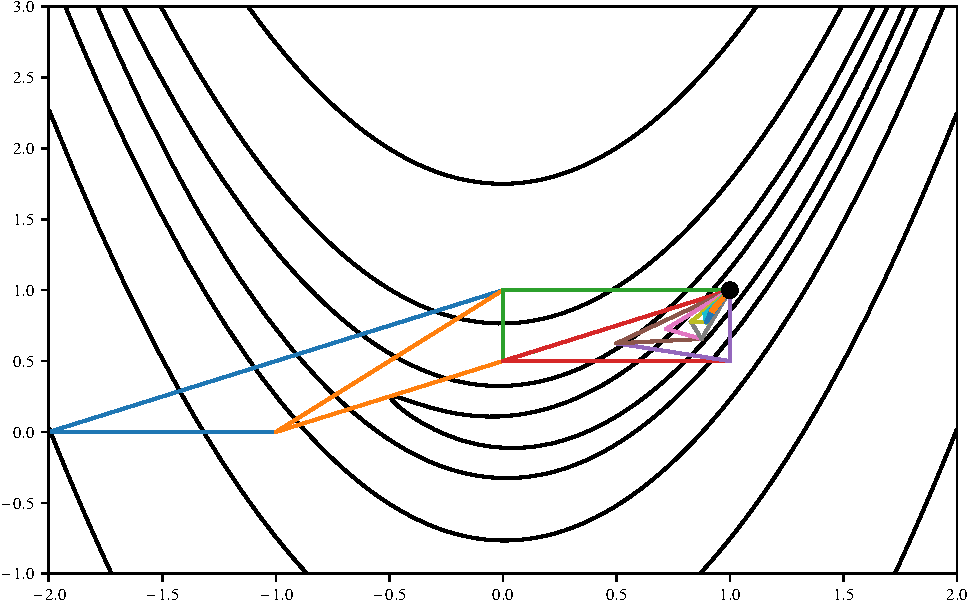
\includegraphics[width=0.75\textwidth]{bannana.pdf}
    \caption{Example of Nelder-Mead method on the Rosenbrock function. Global minimum is at (1,1), as represented by the black dot. Initial simplex is the blue triangle.}
    \label{fig:bannana}
\end{figure}


%AF Code works, tested against toy model, may need further validation. 

%No paper or aim for project. Need contact with Dundee/Ninewells to proceed.

\section{Validation}
\section{Practical application}
\section{Conclusion}